\documentclass[uplatex,dvipdfmx,12pt,nomag]{jsarticle}

\usepackage[a4paper,margin=25mm]{geometry}
\usepackage{amsmath,amssymb}
\usepackage{bm}
\usepackage[dvipdfmx]{graphicx}
\usepackage{float}
\usepackage{framed}
\usepackage{tikz}
\usepackage{xcolor}
\usepackage{listings}
\usepackage[dvipdfmx]{hyperref}
\usepackage{pxjahyper}

\hypersetup{
  colorlinks=true,
  linkcolor=blue,
  urlcolor=blue
}

\lstset{
  language=Python,
  basicstyle=\ttfamily\small,
  keywordstyle=\color{blue!60!black},
  commentstyle=\color{green!40!black},
  stringstyle=\color{red!55!black},
  numbers=left,
  numberstyle=\scriptsize\color{gray},
  stepnumber=1,
  numbersep=0.7em,
  frame=single,
  breaklines=true,
  columns=fullflexible,
  keepspaces=true,
  showstringspaces=false
}

%\setlength{\parindent}{1em}
%\setlength{\parskip}{0.6em}

\newcounter{question}
\newenvironment{questionbox}
  {%
    \refstepcounter{question}%
    \vspace{0.8em}%
    \begin{framed}%
    \noindent\textbf{問\thequestion}\par\smallskip
  }
  {%
    \end{framed}%
    \vspace{0.2em}%
  }

\title{課題演習A1: コンプトン散乱の測定}
\author{鈴木惇也}
\date{2026-04}

\begin{document}

\maketitle

\section{コンプトン散乱の測定についての概略}

\begin{figure}[H]
  \centering
  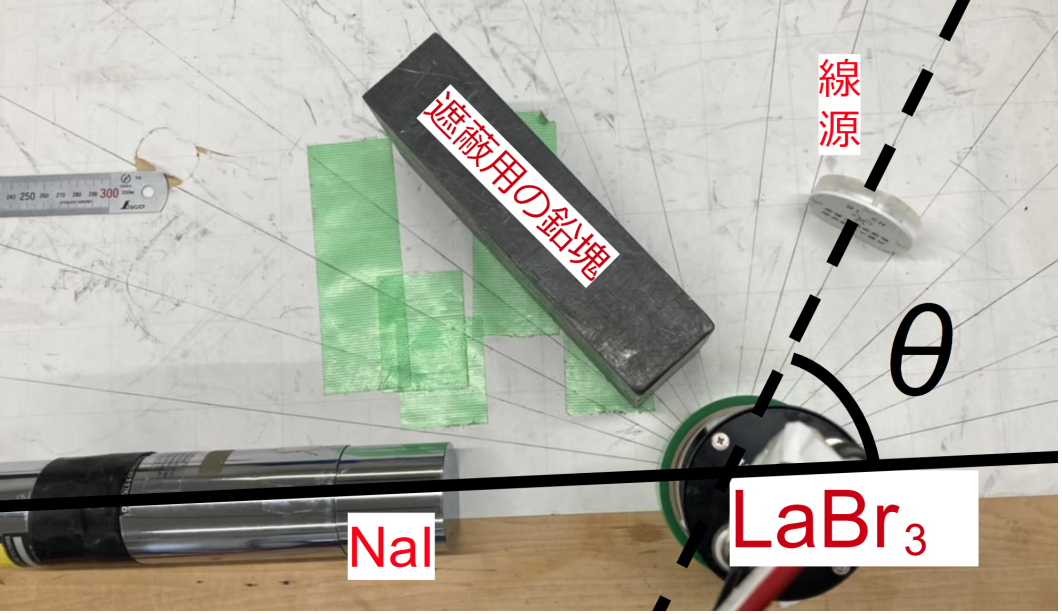
\includegraphics[width=0.62\textwidth]{figures/setup-photo.png}
  \caption{コンプトン散乱測定の配置例\cite{kyoto-a1report22a}}
\end{figure}

コンプトン散乱の実験は図のような要領で行う。まず、$^{137}\mathrm{Cs}$ 放射線源から出た
662\,keV のガンマ線を $\mathrm{LaBr}_{3}(\mathrm{Ce})$ シンチレータに入射させる。ここでコンプトン散乱が
起こると、$\mathrm{LaBr}_{3}(\mathrm{Ce})$ 中の電子が弾かれてシンチレータ中を少しだけ動きエネルギーを落とす
とともに、散乱後のガンマ線も出てくる。

ガンマ線は透過力がある程度高いので、電子と違いシンチレータを突き抜けて出てくるものも多い。
このガンマ線をNaIシンチレータで捉えることで、コンプトン散乱を選択的に測定する。

NaIシンチレータでコンプトン散乱後のガンマ線を完全に吸収できれば、エネルギー保存則により、
$\mathrm{LaBr}_{3}(\mathrm{Ce})$シンチレータとNaIシンチレータで測定したエネルギーの和は、元のガンマ線の
662\,keV と一致する。そこで、次の条件を課すことでコンプトン散乱された事象を選び出す。

\begin{enumerate}
  \renewcommand{\labelenumi}{（\arabic{enumi}）}
  \item $\mathrm{LaBr}_{3}(\mathrm{Ce})$シンチレータとNaIシンチレータが同時に発光すること。
  \item $\mathrm{LaBr}_{3}(\mathrm{Ce})$シンチレータとNaIシンチレータで取得されたエネルギーの和が662\,keV程度になること。
\end{enumerate}

こうした条件を判定するために、同時に発光した事象を選び出す「コインシデンス」と、発光信号波形
（のエネルギーを知るのに必要な情報）を記録して保存する「アナログ-デジタル変換」、信号の値を
エネルギーに変換するための「キャリブレーション」が必要となる。

運動学的な考察から、コンプトン散乱後のガンマ線のエネルギーは、散乱角度に依存することがわかる。
本実験ではこのエネルギーの角度依存性を、実験装置の配置を変更しながら複数回測定することで検証する。
また、コンプトン散乱の断面積は量子電磁気学を用いた理論計算により導出でき、「クライン・仁科の式」という
公式で記述できることがわかる。この散乱断面積の角度依存性の測定も目指す。

\begin{questionbox}
コンプトン散乱後のガンマ線のエネルギーや弾かれた電子のエネルギーの、散乱角度依存性を導出しよう。
（高校でやったかも？）弾かれた電子に与えられたエネルギーの最大値は、入射ガンマ線のエネルギーに対して
どうなるか。
\end{questionbox}

\section{予備実験1: PMTとシンチレータを用いた放射線計測}

この予備実験では、PMTに接続された無機シンチレータにガンマ線を入射し、そのときに現れる電気信号を
オシロスコープで実際に観測する。コンプトン散乱の本測定に入る前に、まず「放射線がシンチレータに入ると何が起こるのか」、
「その結果としてPMTからどのような信号が出てくるのか」、「オシロスコープでは何を見ればよいのか」を
一つずつ確認しておくことがこの予備実験の目的である。

本実験ではオシロスコープを用いて、波形の高さ、幅、立ち上がり、減衰のしかたまで含めて
信号を理解する。
後で行うコインシデンス測定やエネルギー測定では、検出器の応答時間が回路の構成に大きく影響する。
そのため、単に「信号が来た」ということを確認するだけでなく、波形の高さや時間特性を理解しておこう。

\subsection{シンチレータの概略}

シンチレータは、入射した放射線が物質中で失ったエネルギーを、可視光や紫外光として取り出すための物質である。
放射線そのものは目に見えず、またそのまま電気信号として扱うことも容易ではない。しかし、放射線が物質中で
エネルギーを落としたことを光として変換できれば、その光をさらに電気信号へ変えて測定に使うことができる。
後で見るように「光電子増倍管」やゼミで行うシリコンフォトダイオードのような光を電気に変える装置は高性能なものが出ており、
これによって微小なエネルギーの現象も検出できるようになっている。

放射線がシンチレータに入射すると、物質中の電子との相互作用を通してエネルギーを失う。その結果として
シンチレータの準位に励起された状態ができ、最終的に基底状態へ戻る過程で光が放出される。この光の量は、放射線がシンチレータ内に
残したエネルギーとある程度対応しているため、光の強さを測ることによって放射線のエネルギーに関する情報を
得ることができる。放出された光はPMTに導かれ、そこで増幅されて電圧パルスとして観測される。

シンチレータは大きく分けると、無機シンチレータと有機シンチレータに分類される。無機シンチレータは、一般に
密度が高く、また比較的原子番号の大きい元素を含むため、ガンマ線に対してエネルギーを受け止めやすいという特徴がある。
そのため、入射したガンマ線がシンチレータ内でどれだけエネルギーを失ったかを測る用途、特にエネルギースペクトルを
取りたい場合に向いている。一方で、発光の減衰時間は比較的長めであることが多く、非常に高速な時間応答だけを
重視する用途では不利になることもある。

これに対して有機シンチレータは、発光が速く時間分解能に優れるという長所を持つ。したがって、粒子がいつ通過したかを
できるだけ正確に知りたい場合や、高い計数率でイベントをさばきたい場合に有用である。しかし、低原子番号元素が
主体であるためガンマ線を完全に吸収しにくく、全吸収ピークをきれいに観測したいようなエネルギー測定には
あまり向いていない。このように、無機シンチレータと有機シンチレータは優れている点が異なり、目的に応じて
使い分ける必要がある。

本実験で用いるNaI(Tl)シンチレータと$\mathrm{LaBr}_{3}(\mathrm{Ce})$シンチレータも、どちらも無機シンチレータである。
ただし、同じ無機シンチレータでも応答にはかなり違いがある。NaI(Tl)は古くから広く使われてきた代表的な
シンチレータであり、発光量が大きく、比較的扱いやすい。そのため、ガンマ線スペクトルを観測する装置として
教育実験でもよく使われる。一方で、吸湿性があるため取り扱いには注意が必要であり、また発光の時間応答は
それほど速くない。

これに対して$\mathrm{LaBr}_{3}(\mathrm{Ce})$は、Ceを添加した臭化ランタン系のシンチレータであり、
発光が速く、時間分解能に優れている。またエネルギー分解能も良好で、比較的小さなエネルギー差も見分けやすい。
そのため、ある時刻に同時に起こった事象を選びたいコインシデンス測定との相性がよい。

ガンマ線が物質内で起こす主な相互作用としては、光電効果、コンプトン散乱、電子・陽電子対生成の 3 つがよく挙げられる。
これらはどれも「ガンマ線が物質にエネルギーを渡す」という点では共通しているが、その渡し方が異なる。

光電効果では、ガンマ線が原子中の電子にエネルギーをまとめて与え、自身は消滅する。つまり、ガンマ線の持っていた
エネルギーがほぼそのまま物質内に残る。このため、シンチレータがそのエネルギーを十分に受け止めることができれば、
スペクトルには入射エネルギーに対応したはっきりしたピークが現れる。これが光電ピークである。

コンプトン散乱では、ガンマ線は電子にエネルギーの一部だけを与えて向きを変え、自身はより低いエネルギーのガンマ線として
残る。したがって、シンチレータ側に残るエネルギーは事象ごとに変化し、スペクトルとして見ると連続分布を作る。
今回の本実験で中心となるのはまさにこの過程であり、散乱角度とエネルギーの関係を調べることでコンプトン散乱の
特徴を直接確かめることができる。

電子・陽電子対生成は、ガンマ線のエネルギーが十分に高いときに起こる反応で、原子核の近くで電子と陽電子の対が
生成される。対を作るためには少なくとも電子 2 個分の静止質量エネルギーが必要なので、閾値は$2m_{\mathrm e}c^2=1.022\,\mathrm{MeV}$である。
しかし、今回用いる$^{137}\mathrm{Cs}$の主なガンマ線エネルギーは
662\,keV であり、この値は閾値より低い。したがって、この実験で主要な相互作用として考えるべきものは、光電効果とコンプトン散乱である。

\begin{questionbox}
電子・陽電子対生成は真空中でも起こるか？　
四元運動量保存の観点から考えてみよう。
\end{questionbox}

\subsection{光電子増倍管の概略}

\begin{figure}[H]
  \centering
  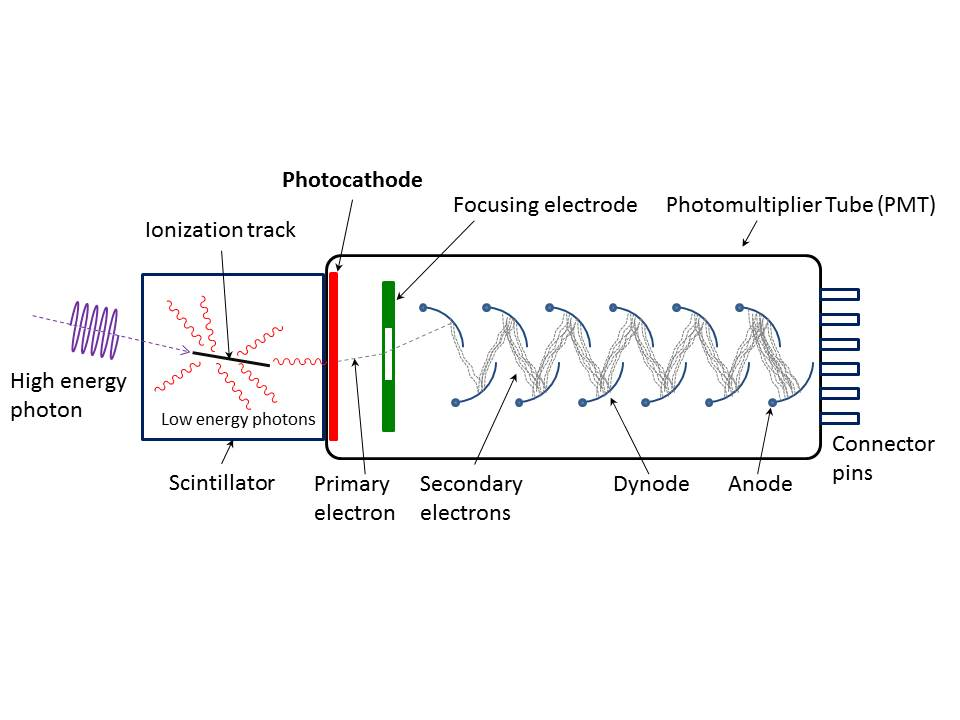
\includegraphics[width=0.8\textwidth,clip,trim=8 150 24 100]{figures/pmt-scintillator-wikimedia.jpg}
  \caption{シンチレータと光電子増倍管の模式図\cite{wikimedia-pmt}}
  \label{fig:pmt-wikimedia}
\end{figure}

光電子増倍管（PMT: Photomultiplier Tube）は、シンチレータから出た弱い光を電気信号へ変換し、それを大きく
増幅する装置である。シンチレータから出る光は非常に弱く、そのままでは扱いにくい。しかしPMTを使うと、
わずかな光でも十分に大きな電圧パルスとして取り出すことができるため、放射線検出器と組み合わせて広く使われている。

PMTの入射窓から入った光は、内部の光電面に到達する。そこで光電効果によって光電子が放出されると、その電子は
高電圧で加速されながらダイノードと呼ばれる電極列に順に衝突する。各ダイノードでは二次電子が複数個放出されるので、
段を経るごとに電子数が増えていく。この増倍過程によって、最初はごく少数しかなかった光電子が最終的には
非常に大きな電荷パルスとなり、陽極から取り出される。

このようにPMTは、単に光を電気に変えるだけではなく、同時に大きな増幅を担っている。
PMTの出力波形は、シンチレータの発光時間特性、PMT自身の応答、信号ケーブル、終端条件など多くの要素によって
決まる。

\subsection{\texorpdfstring{放射線源 $^{137}\mathrm{Cs}$}{放射線源 137Cs}}

本実験で用いる $^{137}\mathrm{Cs}$ はガンマ線測定でよく用いられる標準的な放射線源である。
$^{137}\mathrm{Cs}$ はベータ崩壊によって $^{137}\mathrm{Ba}$ の励起状態を経由し、その脱励起に伴って
主に662\,keVのガンマ線を放出する。このエネルギーは、NaI(Tl)や$\mathrm{LaBr}_{3}(\mathrm{Ce})$のような無機シンチレータで
十分に観測しやすく、かつコンプトン散乱や光電効果の両方が明瞭に現れるため、検出器応答の確認や較正、
散乱実験の線源として適している。

\begin{figure}[H]
  \centering
  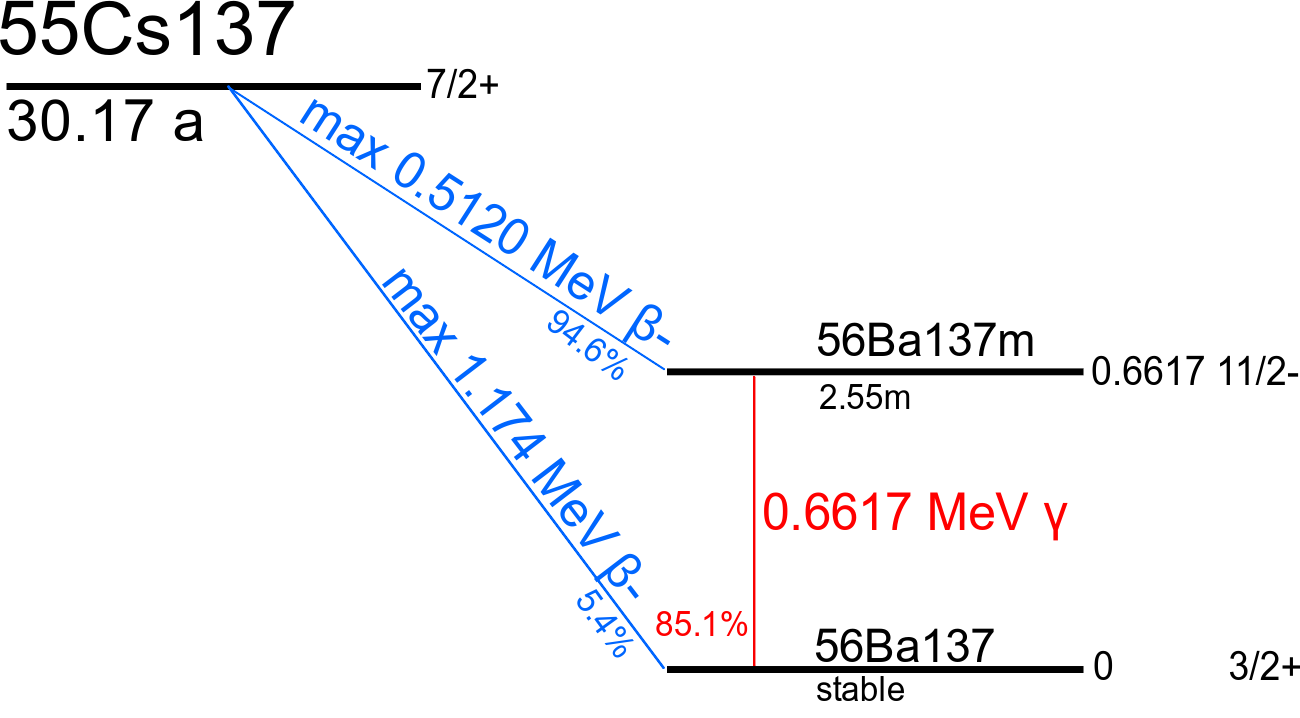
\includegraphics[width=0.6\textwidth]{figures/cs137-decay-wikimedia.png}
  \caption{$^{137}\mathrm{Cs}$ の崩壊図\cite{wikimedia-cs137}}
  \label{fig:cs137-decay}
\end{figure}

図\ref{fig:cs137-decay} に示されるように、$^{137}\mathrm{Cs}$ は主としてベータ崩壊によって
$^{137\mathrm{m}}\mathrm{Ba}$ を経由し、その後の遷移で 661.7\,keV のガンマ線を放出する\cite{wikimedia-cs137}。
実験でしばしば「662\,keV のガンマ線」と表記するのは、この 661.7\,keV の線を丸めて表しているためである。

\subsection{オシロスコープを用いた観測}

オシロスコープは、電圧が時間とともにどのように変化するかを直接見るための装置である。予備実験では、
PMTの出力をオシロスコープに入力し、どのようなパルスが現れるかを観察する。ここで見るべきなのは、
単にパルスの有無だけではない。パルスの高さがどの程度か、立ち上がりが速いか遅いか、減衰がどのくらい長く続くか、
波形のベースラインが安定しているか、といった点を意識しながら観測することが大切である。

基本的な測定では、縦軸を電圧、横軸を時間として表示する。縦軸の感度を適切に選ばないと波形が小さすぎて見えなかったり、
逆に振り切れてしまったりする。また横軸の時間幅を適切に選ばないと、立ち上がりだけしか見えなかったり、
波形の細かな構造がつぶれてしまったりする。さらに、安定して同じような波形を表示するためにはトリガーの設定も重要である。
このように、オシロスコープ観測は単に画面を見るだけではなく、何を見たいのかに応じて測定条件を調整する作業でもある。

信号伝送では50\,$\Omega$終端を用いる。オシロスコープや同軸ケーブルは通常50\,$\Omega$系で
設計されているため、終端条件がこれと合っていないと、信号の一部が端で反射してしまう。反射が起こると、本来 1 回だけ
現れるはずのパルスの後ろに余分な構造が重なったり、波形が振動したりして、真のパルス形状が見えにくくなる。
特に立ち上がりや減衰時間を見たいときには、このような歪みは無視できない。

50\,$\Omega$終端を入れることで、ケーブルと観測器のインピーダンス整合が取れ、信号反射を抑えたより素直な波形を
観測しやすくなる。ただし、その代わりに観測される電圧は小さくなる。したがって、終端を入れればそれでよいという
わけではなく、終端の有無によって波形がどう変わるか、そしてどの設定が目的に合っているかを考えながら測定することが
大切である。
インピーダンスについてはAppendixも参照してみよう。

\begin{questionbox}
「ディバイダー」というモジュールでは、入力された信号の電圧を1/2にしながら2分割を行なっている。
インピーダンス整合の観点から、どのような回路構成になっていると考えられるか。
また、出力側では電圧が1/2になっていることから2つの出力を合わせてもエネルギーは入力の1/2になってしまっている。
このエネルギーはどこに行っているのか。
エネルギーを保存するディバイダーを作ることはできるだろうか。
\end{questionbox}

\subsection{実験のセットアップ}
実験では、PMTに接続されたシンチレータをオシロスコープに接続して波形を観測する。
PMTへは(1)高電圧の供給と(2)信号線の配線を行う。
信号線はPMTの出力端子からオシロスコープの入力端子へ同軸ケーブルで接続する。
オシロスコープの入力は高インピーダンスになっているので、反射を防ぐためには50$\Omega$終端抵抗を並列に入れる必要がある。

実験室には2種類のPMTがある。1つは正の高電圧をかけるタイプ、もう一つは負の高電圧をかけるタイプである。
NaI(Tl)には正、$\mathrm{LaBr}_{3}(\mathrm{Ce})$には負の高電圧をかけるタイプのPMTがつながっている。
ホワイトボードに書かれた標準電圧を参考にしながら、ゆっくりPMTに高電圧をかけていく。
この時、負の高電圧をかけるタイプのPMTでは終端抵抗を除いて1 M$\Omega$で測定しながら、徐々に電圧を上げていこう。
こうすることで光漏れのチェックを簡易的に行うことができる。

オシロスコープの使い方については１回生の実験でやったことを思い出しながら、縦軸の感度、横軸の時間幅、トリガーの設定などを調整して、安定して波形が表示されるようにする。
PMTの信号は負のパルスとして現れる。そのため、オシロスコープのトリガーはfalling edgeで設定する。

NaI(Tl)と$\mathrm{LaBr}_{3}(\mathrm{Ce})$、それぞれに放射線源を当ててみて、信号波形がどのようになっているか記録しよう。
オシロスコープの画面をもとにノートに波形をスケッチし、縦軸のスケールや横軸のスケールを書き込もう。

\begin{questionbox}
正の高電圧をかけるタイプと負の高電圧をかけるタイプのPMTについて、高電圧を分配する「ブリーダー回路」の違いを調べてみよう。
どのような性質の違いがあるだろうか？　
負の高電圧をかけるタイプのPMTで、上述のような光漏れチェックができるのはなぜ？
\end{questionbox}

\section{予備実験2: ディスクリミネータとカウンターを用いた放射線計数}

予備実験2では、予備実験1で見たPMT出力のアナログ波形を、そのまま眺めるだけでなく「何回信号が来たか」を
数えるための電子回路へつなげていく。ここで重要になるのが、NIMモジュール群を用いた回路構成である。
実際の放射線計測では、検出器から出てくる微弱なアナログ信号をそのまま扱うのではなく、必要に応じて
整形し、しきい値を設け、論理信号へ変換してからイベント数を数えたりコインシデンスを組んだりする。
この予備実験では、その最も基本的な流れを体験し、測定系がどのように組まれているかを理解する。

\subsection{NIMモジュールとNIMビン}

本実験で用いる電子回路は、NIM（Nuclear Instrument Module）規格のモジュールを組み合わせて構成する。
NIMモジュールは、それぞれが特定の機能を持つ独立した装置であり、たとえばディスクリミネータ、カウンター、
ゲートジェネレータ、コインシデンス回路などを必要に応じて差し込んで使う。
こうしたモジュールを収める箱を「NIMビン」と呼んでいる。
NIMビンは単なる収納箱ではなく、各モジュールに動作電源を供給する役割も持っている
（実際に端子を見てみよう）。

測定回路は、必要なモジュールをNIMビンに並べ、それらを同軸ケーブルで接続して組み立てる。今回用いる結線には
LEMOコネクタ付きの同軸ケーブルを使う。LEMOは実験系で広く使われる着脱しやすいコネクタであり、
高周波信号やパルス信号を比較的安定に伝送できる（脱着の練習をしてみよう）。

\subsection{ディスクリミネータの役割}

ディスクリミネータは、アナログパルスの高さがある値を超えたときだけ、決まった大きさ・幅の論理信号を出力する回路である。
PMTの出力には、実際に放射線が入射したときの信号だけでなく、電子回路由来のノイズや暗電流に起因する小さな揺らぎも
含まれている。そのため、単に「何か電圧変化があったから 1 回」と数えてしまうと、ノイズまで数えてしまい、
意味のある計数にならない。そこでディスクリミネータを用い、あるしきい値（スレッショルド）以上のパルスだけを
「有効なイベント」として通す。

ディスクリミネータで最も重要な設定のひとつがスレッショルドである。スレッショルドを低くしすぎるとノイズまで
通してしまい、計数率が不自然に大きくなる。一方で高くしすぎると、本来数えたい小さな信号まで切り捨ててしまい、
真の計数率を過小評価することになる。したがって、しきい値設定は「ノイズを除きつつ、実際の信号はできるだけ失わない」
ように調整する必要がある。モジュールによっては出力パルス幅や極性なども設定できるが、まずは
「アナログ信号を論理信号へ変える回路」であると理解するとよい。

\subsection{カウンターの役割}

カウンターは、ディスクリミネータなどから送られてきた論理パルスを数える装置である。一定時間のあいだに
何回パルスが入ったかを記録することで、放射線がどれくらいの頻度で検出されたかを調べることができる。
オシロスコープは個々の波形の形を見るのに適しているのに対し、カウンターは多数のイベントを統計的に扱うのに向いている。
今回の予備実験では、検出器の前に放射線源を置いたとき、距離に応じて検出回数がどのように変化するかを調べるために
カウンターを用いる。

また、放射線計測では統計ゆらぎも本質的に含まれるため、カウント数の大小だけを見るのではなく、測定値にばらつきがあることも
念頭に置いてデータを扱う必要がある。

\subsection{予備実験として行う測定}

この予備実験では、放射線源とシンチレータの距離をいくつか変えながら、毎回同じ測定時間でカウント数を測定する。
距離を近づけるとシンチレータに入射するガンマ線の数は増え、遠ざけると減ると予想される。そこで、距離を段階的に変えつつ
計数を行い、距離とカウント数の関係をデータとして得る。

理想的には、点状線源から等方的に放射線が放出されるならば、単位面積あたりに届く放射線の強さは距離の二乗に反比例して減少する。
したがって、十分に理想化された条件では、計数率もおおむね距離の二乗に反比例して減ることが期待される。
ただし、実際の実験では、線源や検出器が有限の大きさを持つこと、周囲からの散乱による効果があること、検出器の有効面積やしきい値設定の
影響を受けることなどから、完全に理想どおりにはならないことも多い。

解析では、各距離におけるカウント数あるいは計数率をプロットし、距離が大きくなるにつれてどのように減少していくかを確かめる。
必要に応じて背景計数を差し引いたり、横軸を距離 $r$、縦軸を計数率 $N$ として $N \propto 1/r^2$ との比較を行ったりすることで、
単なる感覚的な確認ではなく、定量的に逆二乗則との一致の程度を議論できる。

\section{予備実験3: チャージ積分ADCを用いたスペクトル測定}

予備実験3では、検出器から出てきた信号を単に目で見たり回数を数えたりするだけでなく、コンピュータに取り込んで
数値データとして保存し、エネルギースペクトルとして解析することを学ぶ。ここで中心になるのが、
CAMAC規格のチャージ積分ADCである。シンチレータとPMTの組み合わせから出てくるパルスは、放射線が検出器内に
残したエネルギーに応じて大きさが変化する。そのため、各事象についてパルスの大きさを数値化できれば、
どのようなエネルギーの事象がどれだけ現れたかを分布として調べることができる。

\subsection{放射線スペクトルの形}

ガンマ線源をシンチレータで測定したとき、得られるスペクトルは単純な一本線にはならない。もしすべてのガンマ線が
常に検出器内で全エネルギーを失うなら、入射エネルギーに対応する鋭いピークだけが見えるはずである。しかし実際には、
光電効果だけでなくコンプトン散乱も起こるため、連続成分とピーク成分が重なった形のスペクトルになる。

特に重要なのが、光電ピークとコンプトンエッジである。光電ピークは、ガンマ線が光電効果によってほぼ全エネルギーを
検出器内に残したときに現れるピークであり、線源のエネルギーを知る上で最も基本的な特徴である。一方、コンプトン散乱では
ガンマ線がエネルギーの一部だけを電子に渡して外へ逃げることがあるため、スペクトルには低エネルギー側に連続成分が現れる。
その連続成分の上限に対応する特徴的な端がコンプトンエッジである。これは、コンプトン散乱で電子に与えられるエネルギーが
ある最大値を持つことに由来している。

したがって、スペクトルを見るときには「どこが全吸収ピークなのか」「どこまでがコンプトン連続成分なのか」を意識することが
重要である。こうした特徴を読み取れるようになると、どの反応が主に起きているか、検出器がどの程度エネルギー情報を保持して
いるかを理解しやすくなる。

\subsection{デジタル変換の必要性とADCの種類}

オシロスコープで波形を見ているだけでは、個々の事象の大きさを大量に蓄積して後から統計的に扱うことは難しい。
また、紙にメモを取りながら多数のイベントを処理するのも現実的ではない。そこで必要になるのが、アナログ信号を
デジタル値へ変換し、コンピュータに保存する仕組みである。これによって、各イベントごとの信号強度を数値として保持でき、
ヒストグラム化、フィッティング、較正などの解析が可能になる。

アナログ信号のデジタル化にはいくつかの方法がある。たとえばFlash ADC（高速ADC）を用いると、波形を時間ごとに細かく
サンプリングして、波形そのものをデジタルデータとして記録できる。この方法では立ち上がり、パルス幅、複数ピークの重なりなど、
波形の詳細な時間構造まで後から解析できる。一方で、扱うデータ量は大きくなりやすい。

これに対してチャージ積分ADCは、一定時間内に入力されたパルスの電荷量、すなわち波形の面積に相当する量を1つの数値に
変換する装置である。シンチレータ出力では、パルスの面積が検出器に残されたエネルギーとよく対応することが多いため、
エネルギースペクトルを測定したい場合には非常に使いやすい。今回の予備実験では、波形全体を記録するのではなく、
各イベントの電荷量を 1 イベント 1 データとして取り込むことで、効率よくスペクトルを得る。

\subsection{CAMACについて}

今回のデータ取り込みにはCAMAC（Computer Automated Measurement And Control）規格のモジュールを用いる。
CAMACは、測定用電子回路をモジュール化し、コンピュータから制御・読み出しを行うための規格であり、長年にわたって
原子核・粒子・放射線計測で広く使われてきた。NIMが主としてアナログ回路や論理回路を組み合わせるための規格であるのに対し、
CAMACはデータ取り込みや読み出し、制御といったコンピュータとの接続を担う場面で重要になる。

CAMACクレートには複数のモジュールを挿入でき、その中にADCなどのデータ取得モジュールを組み込む。各モジュールは
スロット番号などで識別され、コンピュータから特定のモジュールを指定してデータを読み出すことができる。
学生実験では内部動作を細かく意識しなくても測定は進められるが、「ADCの値がパソコン画面に出てくる」のは、
背後でCAMACを介した読み出しが行われているからである、という点は理解しておくとよい。

\subsection{光電ピークのガウシアンフィッティング}

実際に得られたスペクトルでは、光電ピークは理想的な鋭い 1 本線にはならず、ある幅を持った山として観測される。
これは、シンチレータの発光統計、PMTの増幅ゆらぎ、電子回路ノイズ、ADCの量子化など、さまざまな要因によって
同じエネルギーの事象でも測定値にばらつきが生じるからである。このようなばらつきが重なると、ピーク形状はしばしば
ガウス分布で近似できる。

そのため、光電ピークの位置を求めたいときには、ピーク近傍をガウシアンでフィッティングする方法がよく用いられる。
フィットによって得られる中心値は、そのエネルギーに対応するADCチャネルの代表値として使うことができる。
また、分布の幅からはエネルギー分解能に関する情報も得られる。

ここでは、\texttt{data} ディレクトリに置いたような「1行に1イベント分のADC値が並んだテキストファイル」を
解析する例として、\texttt{src/fit\_photopeak.py} を用意した。Python環境は \texttt{uv} で作れるようにしてあり、
たとえば $^{137}\mathrm{Cs}$ をNaIで測ったデータなら次のように実行する。

\begin{verbatim}
uv run python src/fit_photopeak.py data/data_137Cs_nai.dat \
  --output figures/photopeak-fit-137Cs-nai.pdf \
  --search-min 1200 --search-max 2200 \
  --fit-half-width 180 \
  --title "137Cs NaI photopeak fit"
\end{verbatim}

スクリプトの最初の仕事は、ADC値を読み込み、指定した幅のヒストグラムに変換することである。
\texttt{np.histogram} は各binに入ったイベント数を返すので、以後のフィットではこのbinごとのカウント数を
データ点として扱う。

\lstinputlisting[firstline=22,lastline=40,caption={ADC値の読み込みとヒストグラム化}]{src/fit_photopeak.py}

ここで注意すべき点は、ヒストグラムの縦軸が「ある一点での確率密度」ではなく
「binの幅に入ったイベント数」だということである。したがってガウシアンをそのままbin中心で評価して
カウント数と比較するのではなく、各binの左端 $a_i$ から右端 $b_i$ まで積分した期待値と比較する。
面積を $A$、中心を $\mu$、標準偏差を $\sigma$ とすると、ガウシアン部分の期待カウント数は
\begin{equation}
  \nu_i^{\mathrm{peak}}
  =
  A \int_{a_i}^{b_i}
  \frac{1}{\sqrt{2\pi}\sigma}
  \exp\left[-\frac{(x-\mu)^2}{2\sigma^2}\right] dx
  =
  \frac{A}{2}
  \left[
  \operatorname{erf}\left(\frac{b_i-\mu}{\sqrt{2}\sigma}\right)
  -
  \operatorname{erf}\left(\frac{a_i-\mu}{\sqrt{2}\sigma}\right)
  \right]
\end{equation}
となる。実際のピークの下にはコンプトン連続成分や背景が少し残るので、コードではこれに一次関数の背景
$c_0+c_1(x_i-x_0)$ を足している。

\lstinputlisting[firstline=43,lastline=64,caption={binごとに積分したガウシアンモデル}]{src/fit_photopeak.py}

このフィットでは、$A$ だけでなく $\mu$ と $\sigma$ もデータから決める。分散は
$\sigma^2$ として得られる。$\mu$ と $\sigma$ は
指数関数や誤差関数の中に入っており、モデルはフィットパラメータに対して線形ではない。
そのため、通常の直線フィットのように連立一次方程式を一度解けば終わり、とはならず、
\texttt{scipy.optimize.curve\_fit} による非線形最小二乗フィットを使う。
非線形フィットでは初期値が収束に影響するので、スクリプトでは次のように初期値を決めている。

\begin{enumerate}
  \renewcommand{\labelenumi}{（\arabic{enumi}）}
  \item \texttt{--search-min} から \texttt{--search-max} の範囲で最もカウントの大きいbinを探し、そこをピーク中心の初期値にする。
  \item その周辺 \texttt{--fit-half-width} の範囲だけをフィットに使う。
  \item フィット範囲の両端の中央値から背景の高さと傾きを見積もる。
  \item 背景を引いた残差の重み付き平均と分散から、$\mu$ と $\sigma$ の初期値を作る。
  \item 背景を引いた残差の和をピーク面積 $A$ の初期値にする。
\end{enumerate}

\lstinputlisting[firstline=67,lastline=98,caption={背景を引いた残差から初期値を作る部分}]{src/fit_photopeak.py}

フィット本体では、各binの統計誤差をポアソン分布のガウス近似
$\sigma_i\simeq\sqrt{N_i}$ として与えている。ただし $N_i=0$ のbinで誤差がゼロになると重みが無限大に
なってしまうため、コードでは \texttt{np.maximum(y, 1.0)} を使って下限を1にしている。
また、面積や幅が負にならないように境界条件を与えている。

\lstinputlisting[firstline=111,lastline=157,caption={ピーク探索と非線形フィットの実行}]{src/fit_photopeak.py}

最後に、ヒストグラムとフィット後の関数を重ね描きしてPDFに保存する。
赤線は連続的なガウス密度を描いたものではなく、表示用の細かい点ごとに
「その幅のbinに入るはずのカウント数」を計算したものである。

\lstinputlisting[firstline=191,lastline=219,caption={ヒストグラムとフィット曲線の重ね描き}]{src/fit_photopeak.py}

\begin{figure}[H]
  \centering
  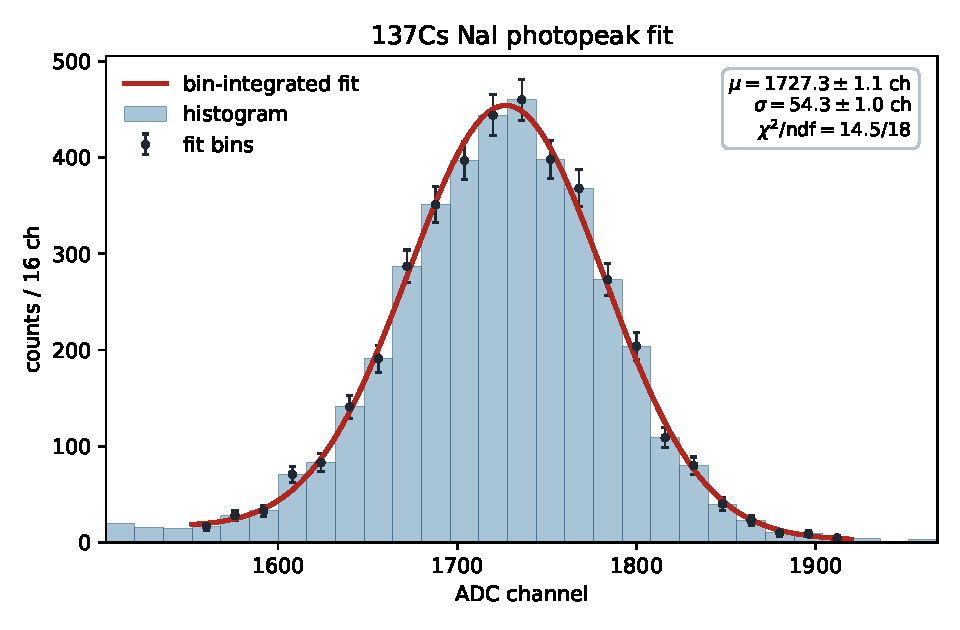
\includegraphics[width=0.74\textwidth]{figures/photopeak-fit-137Cs-nai.pdf}
  \caption{\texttt{data/data\_137Cs\_nai.dat} の光電ピークをbin積分ガウシアンでフィットした例。}
  \label{fig:photopeak-fit-137cs-nai}
\end{figure}

図\ref{fig:photopeak-fit-137cs-nai} の例では、中心は
$\mu = 1727.3\pm1.1$ ch、標準偏差は $\sigma = 54.3\pm1.0$ ch と求まった。
この中心値を、$^{137}\mathrm{Cs}$ の 661.7\,keV の光電ピークに対応するADC値として較正に用いる。
同じ手順を他の線源や他の検出器のデータにも適用し、既知のガンマ線エネルギーとフィットされた中心値を
対応させれば、ADCチャネルからエネルギーへの較正直線を作ることができる。

\subsection{予備実験として行う測定}

この予備実験では、シンチレータとPMTからの信号をチャージ積分ADCに入力し、CAMACを介してコンピュータへ取り込む。
取得されたデータからヒストグラムを作成し、放射線スペクトルを観察する。まずは、どこにコンプトン連続成分が現れ、
どこに光電ピークが現れるかを確認し、検出器がどのような応答をしているかを全体像として把握する。

次に、光電ピーク付近を切り出してガウシアンでフィッティングし、ピーク中心のADC値を求める。これによって、
既知エネルギーを持つガンマ線に対して検出器がどのチャネルに応答するかを定量的に決めることができる。

\section{本実験のセットアップ}

\subsection{シンチレータなどの配置}

\begin{figure}[H]
  \centering
  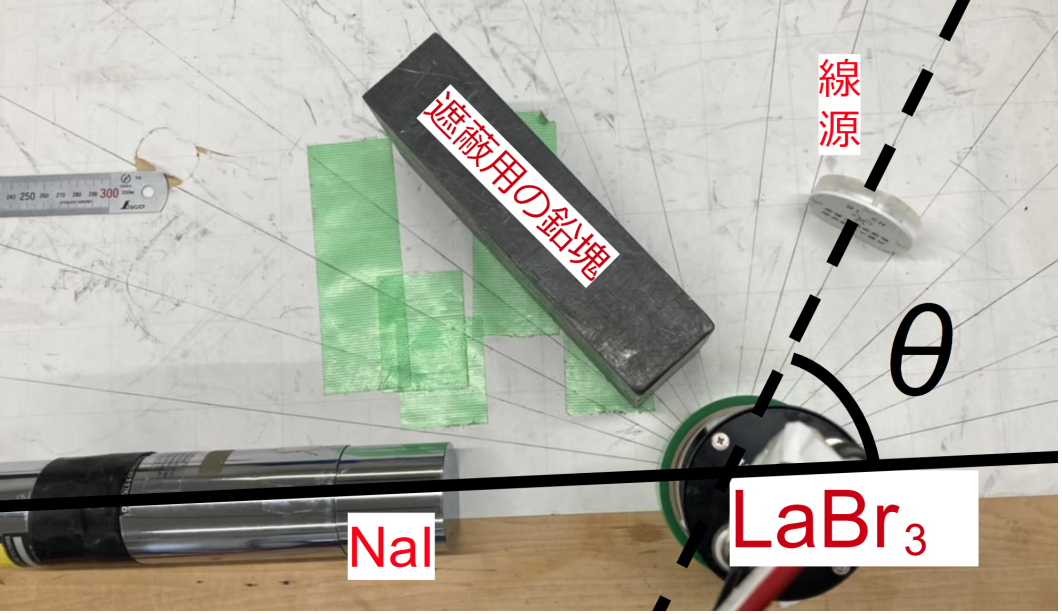
\includegraphics[width=0.78\textwidth]{figures/setup-photo.png}
  \caption{実験セットアップの写真\cite{kyoto-a1report22a}}
\end{figure}

実験は図のようなセットアップで行う。

\begin{enumerate}
  \renewcommand{\labelenumi}{（\arabic{enumi}）}
  \item 分度器のように決まった角度ごとに線の入った紙の上で行うとやりやすい。
  \item $\mathrm{LaBr}_{3}(\mathrm{Ce})$のシンチレータとPMTのセットを鉛直に配置し、分度器の中心に設置する。
  シンチレータとPMTのセットがぐらつかないように、ホルダーとシンチレータの間に発泡スチロールなどを
  挟むとよい。また、シンチレータとPMTは黒いシートで覆われているが、この覆いが取れないように気をつけること。
  \item NaIシンチレータを分度器の0$^\circ$に設置する。
  \item $^{137}\mathrm{Cs}$ 線源を、測定したい角度の場所に置く。この測定したい角度を変えたデータを何点も
  測定し、最終的なデータのセットを得ることになる。（このように線源を動かすのではなく、線源を固定して
  NaIシンチレータを動かしてもよいが、配線も動かさなくてはならなかったりして厄介なので、線源を動かすことの
  方が多い。）
  \item この実験では$\mathrm{LaBr}_{3}(\mathrm{Ce})$でコンプトン散乱されたガンマ線をNaIで測定することを想定している。
  一方、何も遮蔽物がない場合はNaIに$^{137}\mathrm{Cs}$からのガンマ線が入射し、そこでコンプトン散乱した
  散乱ガンマ線が$\mathrm{LaBr}_{3}(\mathrm{Ce})$に入る、という経路も考えられ、邪魔なデータとなる。そこで、遮蔽物（鉛ブロック）を
  置くことでNaIに直接線源から入る経路を遮断する。一方、$\mathrm{LaBr}_{3}(\mathrm{Ce})$でコンプトン散乱された
  ガンマ線が一部でも遮蔽されてしまうと散乱断面積の角度依存性の測定に支障が出るため、その経路に被らないように
  する必要がある。
\end{enumerate}

\begin{questionbox}
プラスチック、鉄、アルミなどではなく鉛ブロックを使う理由は何か。
「NIST XCOM」を使ってそれぞれの材質の662\,keVのガンマ線に対する質量減衰係数
($\mathrm{cm}^{2}/\mathrm{g}$) を調べてみよう。また、密度をかけて $1/e$ になる距離を求めよう。
\end{questionbox}

\subsection{電子回路}

\begin{figure}[H]
  \centering
  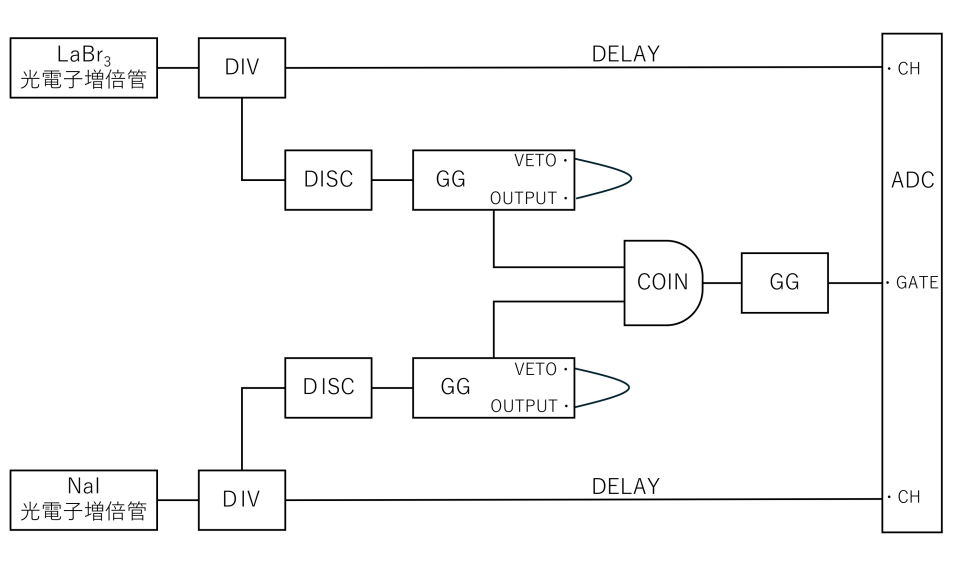
\includegraphics[width=0.92\textwidth]{figures/circuit-diagram.png}
  \caption{電子回路の配線図\cite{kyoto-a1report24a}}
\end{figure}

電子回路は図のように配線する。それぞれのPMTから来た信号は、まずディバイダー（図中「DIV」）により
2分割される。一方の回路は、長い同軸線（「DELAY」）を経由してADC（アナログ-デジタル変換）回路に入力される。

分割されたもう一方の経路は、ディスクリミネータ（「DISC」）に入力され、ある一定の閾値より信号の振幅が
大きかった場合に信号を出力する「トリガー」が作られる。

ディスクリミネータの出力はゲートジェネレータ（「GG」）に入力される。このゲートジェネレータでは
ディスクリミネータの出力したトリガー波形の調整（広くしたり遅延させたり）をする。ゲートジェネレータには
複数の出力があるが、その 1 つをゲートジェネレータの「VETO」に入れることで、「現在ゲートジェネレータが
信号出力をしている時は入力を無視する」ようにすることができる。

それぞれのゲートジェネレータの出力は、コインシデンス（「COIN」）に入力される。コインシデンス回路では
同時に信号が来た時のみ信号を出力する。そのため、概要の（1）にある「同時に発光」したという条件を判定することができる。

このコインシデンスからの信号を再度ゲートジェネレータに入れて整形し、ADCのゲート入力に入れる。
ADCでは信号波形の電荷を積分してデジタル値に変換するが、この積分の範囲をゲート入力で決める。
図のように、オシロスコープでADCに入力される3つの信号をそれぞれ見て、ゲート入力に入る信号が
それぞれのシンチレータからの波形信号を十分カバーできていることを確認してから、データ取得を開始する。

\begin{figure}[H]
  \centering
  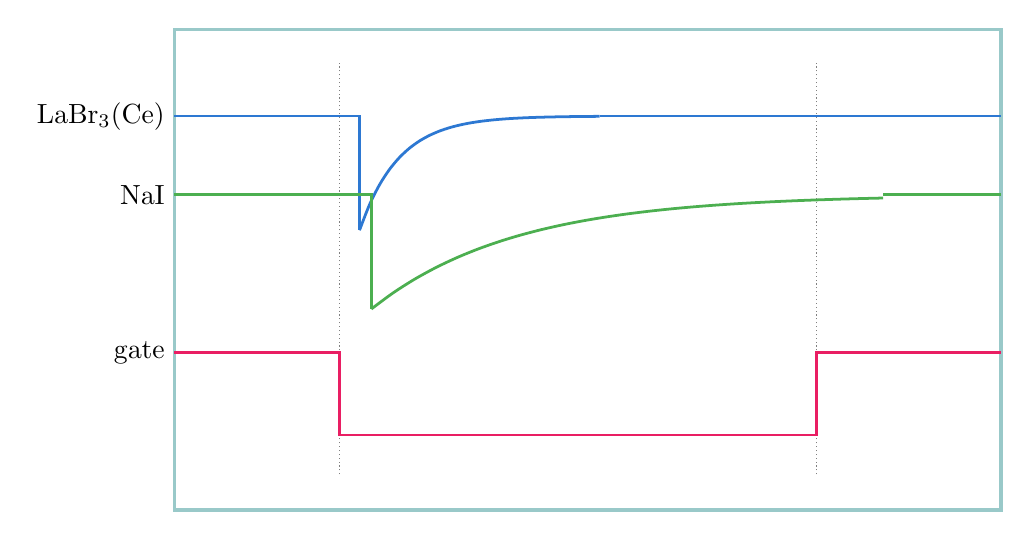
\begin{tikzpicture}[x=1cm,y=1cm]
    \definecolor{framec}{RGB}{153,201,201}
    \definecolor{labr}{RGB}{45,120,210}
    \definecolor{nai}{RGB}{76,175,80}
    \definecolor{gatec}{RGB}{233,30,99}

    \draw[line width=1.3pt, color=framec] (0,0) rectangle (10.5,6.1);
    \draw[densely dotted, gray] (2.1,0.45) -- (2.1,5.7);
    \draw[densely dotted, gray] (8.15,0.45) -- (8.15,5.7);

    \node[left] at (0,5.0) {$\mathrm{LaBr}_{3}(\mathrm{Ce})$};
    \node[left] at (0,4.0) {NaI};
    \node[left] at (0,2.0) {gate};

    \draw[line width=1.0pt, color=labr]
      (0,5.0) -- (2.35,5.0)
      -- (2.35,3.55);
    \draw[line width=1.0pt, color=labr, domain=2.35:5.4, smooth, variable=\x]
      plot ({\x},{5.0 - 1.45*exp(-2.0*(\x-2.35))});
    \draw[line width=1.0pt, color=labr] (5.4,5.0) -- (10.5,5.0);

    \draw[line width=1.0pt, color=nai]
      (0,4.0) -- (2.5,4.0)
      -- (2.5,2.55);
    \draw[line width=1.0pt, color=nai, domain=2.5:9.0, smooth, variable=\x]
      plot ({\x},{4.0 - 1.45*exp(-0.55*(\x-2.5))});
    \draw[line width=1.0pt, color=nai] (9.0,4.0) -- (10.5,4.0);

    \draw[line width=1.0pt, color=gatec]
      (0,2.0) -- (2.1,2.0) -- (2.1,0.95) -- (8.15,0.95) -- (8.15,2.0) -- (10.5,2.0);
  \end{tikzpicture}
  \caption{オシロスコープ模式図}
\end{figure}

\begin{questionbox}
なぜ「DELAY」が必要なのか。また、1メートルの同軸ケーブルに対して何ns（ナノ秒）の遅延が起こるか。
同軸ケーブルの中身の材質の比誘電率を 2.26 として求めてみよう。
\end{questionbox}

\subsection{実験の手順}

\begin{enumerate}
  \renewcommand{\labelenumi}{（\arabic{enumi}）}
  \item 上述のセットアップを組み、ADCに接続される信号をオシロスコープで見て上の図のようになることを確認する。
  \item キャリブレーションを行う。ADCでは電荷量を測定しており、データは0\,pCを「0」、
  1000\,pCを「4095」としてその間を4095分割した値が記録される。この電荷量を計算だけからエネルギーに
  変換するのは困難なため、実測によって変換係数を求める。これが今回の「キャリブレーション（＝較正）」である。
\end{enumerate}

\begin{enumerate}
  \renewcommand{\labelenumi}{（2\alph{enumi}）}
  \item $^{22}\mathrm{Na}$ など $^{137}\mathrm{Cs}$ 以外の線源も持ってくる。複数のエネルギーに対応する点を
  測定することで、切片と傾きを求めることができる。キャリブレーション時はどちらのシンチレータにもガンマ線が入るように、
  鉛の遮蔽を取り除くなど配置を工夫する。
  \item コインシデンス回路はトグルスイッチの設定によって、どの入力のコインシデンスを取るかを変えることができる。
  （通常測定時はNaIと$\mathrm{LaBr}_{3}(\mathrm{Ce})$の両方の入力を使うように設定する。）
  まずはNaIだけを取る設定に変更し、PCでデータ取得を行う。何イベント測定するかは、解析で十分な精度が
  出ているかを見て決める。
  \item 次に$\mathrm{LaBr}_{3}(\mathrm{Ce})$だけを取る設定に変更し、PCでデータ取得を行う。
  \item 線源を別なものに取り替えて（2a）から（2c）の測定を繰り返す。
  \item データを処理して、較正直線を算出する。ガンマ線は光電効果を起こすと（基本的には）全てのエネルギーを
  シンチレータの中に残す。この光電効果の部分のADC値をデータから算出し、ガンマ線のエネルギーと対応づけることで
  較正直線が算出できる。光電効果によるピークを図のようにガウス分布でフィッティングしてガウス分布の中央値を求める。
  こうして求めた値を横軸とし、縦軸にガンマ線のエネルギーを取ると、一つの光電効果のピークについて図で一つの点を打つ
  ことができる。複数のエネルギーについてこれをやることで、直線を引くことができ、この傾きと切片を最小二乗法で求める
  ことで較正直線を得る。この傾きと切片のパラメータを、（3）以降の本測定の解析に用いる。
\end{enumerate}

\begin{figure}[H]
  \centering
  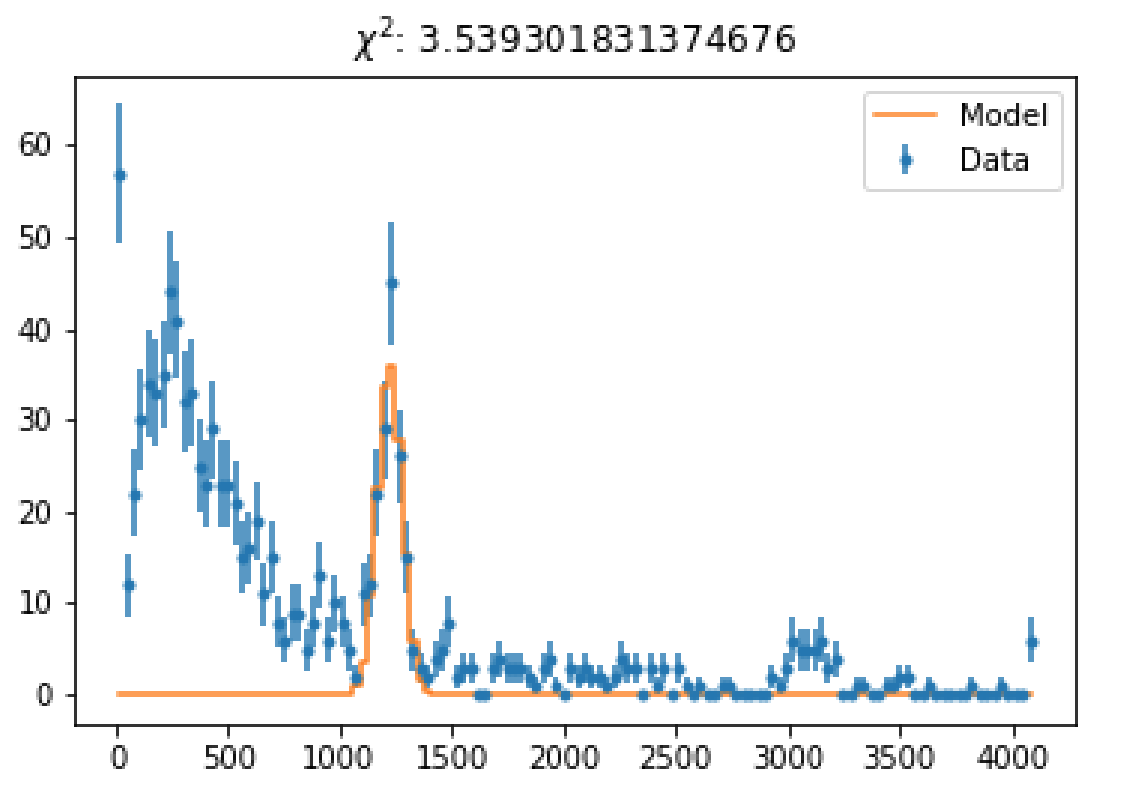
\includegraphics[width=0.60\textwidth]{figures/gaussian-fit.png}\hfill
  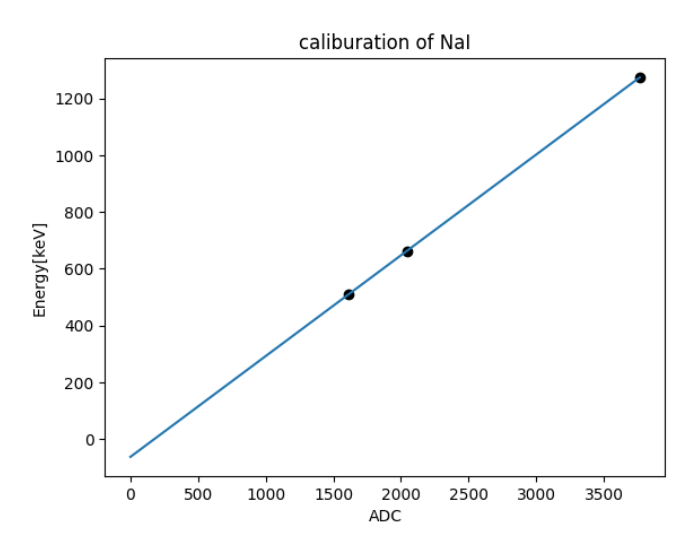
\includegraphics[width=0.36\textwidth]{figures/calibration-line.png}
  \caption{光電ピークのフィッティング例（左）と較正直線の例（右）\cite{kyoto-a1report22a}}
\end{figure}

\begin{enumerate}
  \setcounter{enumi}{2}
  \renewcommand{\labelenumi}{（\arabic{enumi}）}
  \item 測定したい角度 $\theta$ を決めて $^{137}\mathrm{Cs}$ 線源を設置する。鉛の遮蔽を行い、
  望まないデータが入らないように配置する（都度、写真を撮っておくと考察の時に役立つかもしれない）。
  コインシデンスの入力を両方の入力を使うように設定して、本測定を開始する。
\end{enumerate}

\begin{enumerate}
  \renewcommand{\labelenumi}{（3\alph{enumi}）}
  \item 線源の距離が$\mathrm{LaBr}_{3}(\mathrm{Ce})$に近ければ、シンチレータに入射されるガンマ線の数は多くなり
  データが早く貯まりやすくなる。一方、シンチレータの大きさが有限であることから、角度の不定性は大きくなることがわかる。
  この「データの貯まる速度」と「角度の精度」との兼ね合いでセットアップを決める必要がある。
  \item NaIと$\mathrm{LaBr}_{3}(\mathrm{Ce})$との距離でも、同様のことが言える。
\end{enumerate}

\begin{enumerate}
  \setcounter{enumi}{3}
  \renewcommand{\labelenumi}{（\arabic{enumi}）}
  \item 複数の角度 $\theta$ で（3）の測定を繰り返す。
\end{enumerate}

\appendix

\section{CAMAC規格の概要}

このappendixでは、予備実験3で用いたCAMACについて、本文より少し詳しく整理する。学生実験では
「ADCモジュールを挿し、コンピュータから読み出す箱」として使うことが多いが、CAMACはもともと
測定機器をモジュール化し、共通の方法で制御・読み出しするために整備された規格である\cite{ieee583,camac-intro}。

\subsection{CAMACとは何か}

CAMACは\textit{Computer Automated Measurement And Control}の略であり、測定・制御用モジュールを
共通のクレートに収め、標準化されたデータバスを介してコンピュータから制御するための規格である\cite{ieee583}。
NIMが主としてアナログ回路や論理回路を組み合わせるための規格であるのに対し、CAMACは
コンピュータによるデータ取得や機器制御を意識したデジタルインターフェース規格として発展した。

IEEEの標準ページでは、CAMACは機械仕様と信号仕様の両方を定め、異なるメーカーのモジュール同士でも
物理的・機能的に互換性を持てるようにすることを目的としている、と説明されている\cite{ieee583}。
この考え方によって、検出器ごと・計測器ごとに専用配線を一から設計するのではなく、共通のクレートと
共通の通信手順の上でシステムを構築できるようになった。

\subsection{クレートとステーション}

CAMACの基本単位はクレート（crate）であり、その中に複数のモジュールを挿入して用いる。
現在もCAMACクレートを製造しているW-IE-NE-Rの技術説明では、標準的なCAMACクレートは25スロットを持ち、
右端のstation 25はcrate controller用に予約され、通常のモジュールはstation 1から24に挿す、
と説明されている\cite{camac-intro}。また、crate controllerはしばしば二重幅モジュールで、
右端の 24, 25 を使う構成になっている\cite{camac-intro}。

クレートの背面にはDatawayと呼ばれる共通バスが通っており、各モジュールはこのDatawayを介して
電源供給、アドレス指定、制御信号、データ転送を受ける\cite{ieee583,camac-intro}。
本文中で使ったCAMAC ADCも、このクレートに挿さる1つのモジュールであり、単独で完結しているわけではなく、
クレートとcontrollerを含むシステム全体の一部として動いている。

\subsection{Datawayと24ビットデータ}

CAMACの中心にあるのがDatawayである。IEEEの標準概要では、CAMACはDatawayによって
機器・周辺装置・コンピュータ・外部controllerが通信できるように完全なバス仕様を与えている、とされている\cite{ieee583}。
また、W-IE-NE-Rの説明では、CAMAC Datawayは24ビット語を扱うデータ転送線を持ち、
24本のRead線と24本のWrite線、さらにストローブやアドレス・制御線を含む構成である\cite{camac-intro}。

そのため、CAMACモジュールの読み書きは基本的に24ビットデータを単位として行われる。
学生実験で使うADCでも、最終的には「あるイベントに対して24ビット幅の値が返ってくる」という形で
データが扱われる。もちろん実際に有効なビット数はモジュール依存であり、12 bit ADCや16 bit ADCのように
見えることもあるが、CAMACのやり取りそのものは24ビットDataway上で定義されている。

\subsection{\texorpdfstring{$N$-$A$-$F$}{NAF} と \texorpdfstring{$C$-$N$-$A$-$F$}{CNAF}}

CAMACのアクセスでは、どのモジュールに対してどの操作を行うかを、アドレス情報と機能コードの組で指定する。
よく使われる表記が$N$-$A$-$F$である。ここで$N$はstation number、すなわちどのスロットのモジュールかを表し、
$A$ は subaddress、$F$ は function code である\cite{camac-intro}。

技術解説では、$N$は前面から見て左端から始まるstation番号、$A$は4本のアドレス線で指定される
0から15のsubaddress、$F$は5本のfunction線で指定される機能であると説明されている\cite{camac-intro}。
つまりCAMACでは、「どのモジュールの」「どの内部レジスタや機能ブロックに対して」「どの操作をするか」を
明示してコマンドを出すことになる。

複数クレートを扱う系では、crate番号$C$も付けて$C$-$N$-$A$-$F$（CNAF）と書くことが多い\cite{fermilab-camac}。
FermilabのCAMAC解説でも、CNAFはcrate、slot、subaddress、functionを含み、書き込みなら24ビット値を送り、
読み出しなら24ビット値が返る、と説明されている\cite{fermilab-camac}。学生実験ではcrateが1台だけなので
crate番号を意識しないことも多いが、ソフトウェアの内部ではこのような形でアクセスしていると考えると分かりやすい。

\subsection{制御信号と応答}

CAMACでは、データの読み書きだけでなく、クレート全体や各モジュールの状態を扱う制御信号も重要である。
たとえば解説資料では、Dataway上の各コマンド動作にBusy線と2つのストローブ$S1$, $S2$が使われること、
またモジュール側からの状態応答として$Q$信号が返ることが説明されている\cite{camac-intro}。

実務上よく現れるのが、crate initializeを表す$Z$、crate clearを表す$C$、inhibitの設定・解除などである。
またLAM（Look-At-Me）は、モジュール側が「自分に注目してほしい」、すなわち読み出しや処理が必要な状態になったことを
controllerに知らせる仕組みとして使われる\cite{camac-intro}。学生実験ではソフトウェアがこれらを
裏で処理していることが多いが、CAMACが単なるメモリ読み出しではなく、測定器制御のためのバス規格であることは、
こうした信号の存在からも分かる。

\section{インピーダンスの基礎}

このappendixでは、オシロスコープ観測や同軸ケーブル配線で繰り返し現れる「インピーダンス」という概念を整理する。
学生実験では50\,$\Omega$終端や50\,$\Omega$ケーブルという言葉が頻繁に出てくるが、その意味を
理解しておくと、なぜ反射が起きるのか、なぜ終端が必要なのか、なぜ同軸ケーブルの種類が信号品質に影響するのかを
物理的に考えやすくなる。

\subsection{出力インピーダンスと入力インピーダンス}

回路の出力端子は、理想的な電圧源のように「どんな負荷につないでも同じ電圧を出す」わけではない。
実際には、内部にある有限のインピーダンスを持った電源として振る舞う。これを出力インピーダンス
（output impedance）という。簡単なモデルでは、理想電圧源 $V_{\mathrm s}$ に直列に
インピーダンス $Z_{\mathrm out}$ が入っていると考えられる。

一方、信号を受ける側の装置も、入力端子に対してあるインピーダンスを持つ。これを入力インピーダンス
（input impedance）という。たとえばオシロスコープは、1\,M$\Omega$ 入力として使う場合と
50\,$\Omega$ 終端を入れて使う場合とで、信号源から見た負荷条件が大きく変わる。

出力インピーダンス $Z_{\mathrm out}$ の信号源を、入力インピーダンス $Z_{\mathrm in}$ の負荷につないだとき、
負荷側にかかる電圧は単純な分圧として
\begin{equation}
  V_{\mathrm in}
  =
  V_{\mathrm s}
  \frac{Z_{\mathrm in}}{Z_{\mathrm out}+Z_{\mathrm in}}
\end{equation}
と書ける。したがって、入力インピーダンスが十分大きければ信号電圧はほとんど落ちないが、
50\,$\Omega$ 終端のように比較的小さい負荷につなぐと、観測電圧は小さくなる。

\subsection{インピーダンス整合と反射}

直流回路では、単に電圧降下や電流値だけを考えればよいことが多い。しかし、短いパルスや高周波信号を
ケーブルで伝送する場合、ケーブルは単なる導線ではなく伝送線路として振る舞う。このとき重要になるのが、
伝送線路の特性インピーダンス $Z_0$ と、終端側の負荷インピーダンス $Z_{\mathrm L}$ の関係である。

負荷インピーダンスが特性インピーダンスと一致しないと、信号の一部は負荷で吸収されずに反射する。
反射の大きさは反射係数
\begin{equation}
  \Gamma
  =
  \frac{Z_{\mathrm L}-Z_0}{Z_{\mathrm L}+Z_0}
\end{equation}
で表される。たとえば $Z_{\mathrm L}=Z_0$ であれば
\begin{equation}
  \Gamma = 0
\end{equation}
となり、反射は起こらない。これがインピーダンス整合である。

逆に、終端を入れずに高インピーダンス入力へパルスを入れると、$Z_{\mathrm L}$ は $Z_0$ よりかなり大きくなるため、
$\Gamma$ は 1 に近づき、強い反射が起こる。オシロスコープ画面でパルスの後ろに余分な段差や揺れが見えるのは、
この反射波が戻ってきて重なっているためである。パルス波形を正しく見たいときに 50\,$\Omega$ 終端が重要なのは、
まさにこの反射を抑えるためである。

\subsection{同軸ケーブルの形状と特性インピーダンス}

同軸ケーブルは、内導体と外導体が同軸円筒状に配置され、その間を誘電体が満たしている構造を持つ。
この構造から、単位長さあたりのインダクタンス $L'$ とキャパシタンス $C'$ が決まり、損失の小さい近似では
特性インピーダンスは
\begin{equation}
  Z_0 = \sqrt{\frac{L'}{C'}}
\end{equation}
で与えられる。この式は、損失のない伝送線路を記述するテレグラファー方程式
\begin{equation}
  \frac{\partial V}{\partial x} = -L' \frac{\partial I}{\partial t},
  \qquad
  \frac{\partial I}{\partial x} = -C' \frac{\partial V}{\partial t}
\end{equation}
から導かれる。$e^{i(kx - \omega t)}$ 型の進行波解を代入すると $kV = \omega L' I$、$kI = \omega C' V$
が得られ、両式から $V/I = \sqrt{L'/C'}$ となる。これが特性インピーダンスの値を与える。

以下では、同軸ケーブルの幾何学的構造から $L'$ と $C'$ を具体的に求めておく。まずキャパシタンスについて考える。
内導体に単位長さあたり電荷 $\lambda$ があり、外導体に $-\lambda$ があるとする。半径 $r$ の円筒面を
ガウス面にとると、電場は半径方向のみを向き、
\begin{equation}
  E(r)\,2\pi r \ell = \frac{\lambda \ell}{\varepsilon}
\end{equation}
より
\begin{equation}
  E(r) = \frac{\lambda}{2\pi \varepsilon r}
\end{equation}
となる。ここで $\varepsilon=\varepsilon_0\varepsilon_r$ である。したがって、内導体半径 $a$ から
外導体内半径 $b$ までの電位差は
\begin{equation}
  V = \int_a^b E(r)\,dr
    = \frac{\lambda}{2\pi\varepsilon}\int_a^b \frac{dr}{r}
    = \frac{\lambda}{2\pi\varepsilon}\ln\frac{b}{a}
\end{equation}
となる。よって単位長さあたりのキャパシタンスは
\begin{equation}
  C' = \frac{\lambda}{V}
     = \frac{2\pi\varepsilon}{\ln(b/a)}
     = \frac{2\pi\varepsilon_0\varepsilon_r}{\ln(b/a)}
\end{equation}
と求まる。

次にインダクタンスを考える。内導体に電流 $I$ が流れ、外導体に戻り電流 $-I$ が流れているとする。
半径 $r$ の円周をアンペール経路にとると
\begin{equation}
  H(r)\,2\pi r = I
\end{equation}
より
\begin{equation}
  H(r)=\frac{I}{2\pi r}
\end{equation}
であり、磁束密度は
\begin{equation}
  B(r)=\mu H(r)=\frac{\mu I}{2\pi r}
\end{equation}
となる。ここで通常の同軸ケーブルでは誘電体部分の透磁率はほぼ $\mu_0$ とみなせるので $\mu\simeq\mu_0$ とする。
磁気エネルギー密度 $u_{\mathrm m}=B^2/(2\mu)$ を断面で積分すると、単位長さあたりの磁気エネルギー $U'_{\mathrm m}$ は
\begin{equation}
  U'_{\mathrm m}
  = \int_a^b \frac{B(r)^2}{2\mu}\, 2\pi r\,dr
  = \int_a^b \frac{\mu I^2}{8\pi^2 r^2}\,2\pi r\,dr
  = \frac{\mu I^2}{4\pi}\ln\frac{b}{a}
\end{equation}
となる。一方、インダクタンスの定義から
\begin{equation}
  U'_{\mathrm m}=\frac{1}{2}L'I^2
\end{equation}
なので
\begin{equation}
  L'=\frac{\mu}{2\pi}\ln\frac{b}{a}
\end{equation}
を得る。ここで $\mu\simeq\mu_0$ とすれば
\begin{equation}
  L' = \frac{\mu_0}{2\pi}\ln\frac{b}{a}
\end{equation}
となる。

同軸ケーブルでは、内導体半径を $a$、外導体内半径を $b$、誘電体の比誘電率を $\varepsilon_r$ とすると、
真空の透磁率 $\mu_0$、真空の誘電率 $\varepsilon_0$ を用いて
\begin{equation}
  L' = \frac{\mu_0}{2\pi}\ln\frac{b}{a},
  \qquad
  C' = \frac{2\pi\varepsilon_0\varepsilon_r}{\ln(b/a)}
\end{equation}
となる。これを代入すると
\begin{equation}
  Z_0
  =
  \frac{1}{2\pi}\sqrt{\frac{\mu_0}{\varepsilon_0\varepsilon_r}}
  \ln\frac{b}{a}
  =
  \frac{60}{\sqrt{\varepsilon_r}}\ln\frac{b}{a}
\end{equation}
が得られる。常用対数を使えば
\begin{equation}
  Z_0 \simeq \frac{138}{\sqrt{\varepsilon_r}}\log_{10}\frac{b}{a}
\end{equation}
とも書ける。

この式から、同軸ケーブルの特性インピーダンスは、単に材質だけでなく、内導体と外導体の半径比にも依存することが分かる。
つまり、50\,$\Omega$ ケーブルや 75\,$\Omega$ ケーブルという違いは、誘電体の種類と幾何学的寸法の両方によって
決まっている。実験室でよく使う 50\,$\Omega$ 同軸ケーブルは、パルス伝送や計測機器との整合を重視した設計になっている。

\subsection{伝搬速度と遅延}

同軸ケーブル中の信号伝搬速度 $v$ は、損失を無視すれば
\begin{equation}
  v = \frac{1}{\sqrt{L'C'}} = \frac{c}{\sqrt{\varepsilon_r}}
\end{equation}
で与えられる。ここで $c$ は真空中の光速である。したがって、ケーブル長を $\ell$ とすると遅延時間は
\begin{equation}
  t = \frac{\ell}{v} = \frac{\ell\sqrt{\varepsilon_r}}{c}
\end{equation}
となる。

たとえば、予備課題でも使ったように $\varepsilon_r=2.26$ の誘電体を考えると、
\begin{equation}
  v \simeq \frac{3.0\times10^8}{\sqrt{2.26}}
  \approx 2.0\times10^8\ \mathrm{m/s}
\end{equation}
であり、1\,m あたりの遅延は
\begin{equation}
  t \approx \frac{1}{2.0\times10^8}\ \mathrm{s}
  \approx 5.0\ \mathrm{ns}
\end{equation}
程度となる。これは実験で DELAY ケーブルを用いるときの見積もりとも一致する。


\clearpage
\section{解析の基礎: 計数データの統計的取り扱い}

この付録では、予備実験2で行う「距離を変えながらカウント数を測定する」実験を念頭に、
計数データの統計的取り扱いを整理する。

\subsection{二項分布とポアソン分布}

放射性崩壊を例に考える。$N$ 個の原子核があり、ある短い時間内にそれぞれが崩壊する確率が
$p$（$\ll 1$）であるとする。このとき観測される崩壊数 $k$ は\textbf{二項分布}に従い、
\begin{equation}
  P_{\mathrm{bin}}(k;\, N,\, p)
  = \binom{N}{k} p^k (1-p)^{N-k}
\end{equation}
と書ける。ここで平均 $\mu = Np$ を固定したまま $N \to \infty$、$p \to 0$ の極限をとる。
まず二項係数と $p^k$ の積について、
\begin{equation}
  \binom{N}{k} p^k
  = \frac{N(N-1)\cdots(N-k+1)}{k!}
    \left(\frac{\mu}{N}\right)^k
  \xrightarrow{N\to\infty} \frac{\mu^k}{k!}
\end{equation}
また残りの因子は
\begin{equation}
  (1-p)^{N-k}
  = \left(1 - \frac{\mu}{N}\right)^{N-k}
  \xrightarrow{N\to\infty} e^{-\mu}
\end{equation}
以上から\textbf{ポアソン分布}が得られる：
\begin{equation}
  P(k;\, \mu) = \frac{\mu^k\, e^{-\mu}}{k!}
  \label{eq:poisson}
\end{equation}

\subsubsection*{期待値と分散}

期待値は、$k=0$ の項がゼロになることを使うと
\begin{equation}
  \langle k \rangle
  = \sum_{k=0}^{\infty} k\,\frac{\mu^k e^{-\mu}}{k!}
  = \mu e^{-\mu} \sum_{k=1}^{\infty} \frac{\mu^{k-1}}{(k-1)!}
  = \mu
\end{equation}
同様に $\langle k(k-1)\rangle$ を計算すると、
\begin{equation}
  \langle k(k-1) \rangle
  = e^{-\mu}\sum_{k=2}^{\infty}\frac{\mu^k}{(k-2)!}
  = \mu^2 e^{-\mu} \sum_{j=0}^{\infty}\frac{\mu^j}{j!}
  = \mu^2
\end{equation}
したがって分散は
\begin{equation}
  \mathrm{Var}[k]
  = \langle k^2\rangle - \langle k\rangle^2
  = \langle k(k-1)\rangle + \langle k\rangle - \langle k\rangle^2
  = \mu^2 + \mu - \mu^2 = \mu
\end{equation}
となる。すなわちポアソン分布では\textbf{期待値と分散が等しく}、
標準偏差は $\sigma = \sqrt{\mu}$ である。
実験では真の $\mu$ は未知なので、観測値 $N$ を代わりに使い
$\sigma \approx \sqrt{N}$ と推定するのが標準的である。

\subsection{最尤推定によるパラメータ推定}

距離 $r_i$ で測定したカウント数を $N_i$ とする。
点線源からの等方放射を仮定すると、期待カウント数は逆二乗則から
\begin{equation}
  \mu_i = \frac{a}{r_i^2}
  \label{eq:inv-sq}
\end{equation}
と書ける（$a$ は線源強度・測定時間・検出効率などをまとめたパラメータ）。
本当はシンチレータの大きさやバックグラウンドの影響も考慮すべきだが、ここではまずこの式での解析を試みてみよう。

各測定点は互いに独立なポアソン過程とみなせるので、尤度（likelihood）は
\begin{equation}
  L(a) = \prod_{i} P(N_i;\,\mu_i(a))
       = \prod_{i} \frac{\mu_i(a)^{N_i}\,e^{-\mu_i(a)}}{N_i!}
\end{equation}
対数をとると
\begin{equation}
  \ln L(a)
  = \sum_{i} \bigl[-\mu_i(a) + N_i \ln \mu_i(a)\bigr] + \mathrm{const}
  \label{eq:logL}
\end{equation}
最適な$a$の値を求めるため、
$\mu_i = a/r_i^2$ を代入して $a$ で微分し、$\partial \ln L/\partial a = 0$ とおくと
\begin{equation}
  \sum_{i}\left(-\frac{1}{r_i^2} + \frac{N_i}{a}\right) = 0
\end{equation}
これを解くと最尤推定量が解析的に
\begin{equation}
  \hat{a} = \frac{\displaystyle\sum_{i} N_i}{\displaystyle\sum_{i} r_i^{-2}}
  \label{eq:ahat}
\end{equation}
と求まる。

\subsubsection*{パラメータの不確かさ}

$S \equiv \sum_i r_i^{-2}$、$M \equiv \sum_i N_i$ と置くと、式\eqref{eq:logL}に $\mu_i = a/r_i^2$ を
代入した対数尤度は $a$ の具体的な関数として
\begin{equation}
  \ln L(a) = -aS + M\ln a + \mathrm{const}
  \label{eq:logL-concrete}
\end{equation}
と書ける（const は $a$ に依存しない項）。これは $a > 0$ で定義された上に凸な関数であり、
$\partial \ln L/\partial a = -S + M/a = 0$ を解くと最大点 $\hat{a} = M/S$ が得られる（式\eqref{eq:ahat}）。

最大値からのずれを
\begin{equation}
  \Delta\ln L(a) \equiv \ln L(a) - \ln L(\hat{a})
  = -S(a - \hat{a}) + M\ln\frac{a}{\hat{a}}
\end{equation}
とおく。$\hat{a}$ 近傍で $\varepsilon = a - \hat{a}$ として展開すると、
$\ln(1 + \varepsilon/\hat{a}) \approx \varepsilon/\hat{a} - \varepsilon^2/(2\hat{a}^2)$ を使えば、
一次の項（$-S + M/\hat{a} = 0$）が消えて
\begin{equation}
  \Delta\ln L(a) \approx -\frac{M}{2\hat{a}^2}(a - \hat{a})^2
  \label{eq:dlnL}
\end{equation}
となる。$\Delta\ln L(a)$ が $a$ の二次関数になっていることから、
尤度の「幅」としてパラメータの不確かさが自然に読み取れそうである。
では、その幅をどの閾値で切り取ればよいか。以下では、ガウス型尤度を例に
$\Delta\ln L = -1/2$ が $1\sigma$ 区間の境界を与えることを確認する。

\paragraph{$\Delta\ln L = -1/2$ の由来.}
推定量 $\hat{a}$ が真の値 $a$ のまわりでガウス分布 $\hat{a}\sim\mathcal{N}(a,\,\sigma^2)$ に
従うとき、尤度は $a$ の関数として
\begin{equation}
  L(a) \propto \exp\!\left(-\frac{(\hat{a}-a)^2}{2\sigma^2}\right)
\end{equation}
と書ける。対数をとると
\begin{equation}
  \ln L(a) = -\frac{(a - \hat{a})^2}{2\sigma^2} + \mathrm{const}
\end{equation}
であり、最大点 $a = \hat{a}$ からのずれは
\begin{equation}
  \Delta\ln L(a) = -\frac{(a-\hat{a})^2}{2\sigma^2}
\end{equation}
となる。$1\sigma$ 境界 $a = \hat{a} \pm \sigma$ を代入すると
\begin{equation}
  \Delta\ln L(\hat{a}\pm\sigma) = -\frac{\sigma^2}{2\sigma^2} = -\frac{1}{2}
\end{equation}
となる。すなわち、\textbf{ガウス分布の指数の肩にある $1/(2\sigma^2)$ がそのまま $1/2$ として現れる}。
$\Delta\ln L \geq -1/2$ を満たす $a$ の範囲が $[\hat{a}-\sigma,\,\hat{a}+\sigma]$ に等しく、
これが $1\sigma$ 区間を定義する。
尤度がガウス型でない場合も、大標本では Wilks の定理により $-2\Delta\ln L$ が
自由度 1 の $\chi^2$ 分布に漸近するため、同じ基準を用いることができる。

この基準を式\eqref{eq:dlnL}に適用する。$\Delta\ln L = -1/2$ を代入すると
\begin{equation}
  \frac{M}{2\hat{a}^2}(a - \hat{a})^2 = \frac{1}{2}
  \quad\Longrightarrow\quad
  \sigma_{\hat{a}}
  = \frac{\hat{a}}{\sqrt{M}}
  = \frac{\hat{a}}{\sqrt{\sum_i N_i}}
  = \frac{\sqrt{\sum_i N_i}}{\sum_i r_i^{-2}}
  \label{eq:mle-err2}
\end{equation}
が得られる。相対誤差は $\sigma_{\hat{a}}/\hat{a} = 1/\sqrt{M}$ であり、
総カウント数が多いほど推定精度が上がることがわかる。

\paragraph{曲率との対応.}
式\eqref{eq:dlnL}から $\ln L$ の曲率は $-M/\hat{a}^2$ であり、
これをフィッシャー情報量 $I(\hat{a}) = -\partial^2\ln L/\partial a^2\big|_{\hat{a}}$ と呼ぶ。
1パラメータの場合には、推定量の標準偏差はこの曲率の逆平方根として
\begin{equation}
  \sigma_{\hat{a}} = \frac{1}{\sqrt{I(\hat{a})}}
  \label{eq:mle-err}
\end{equation}
と書ける。これは $\Delta\ln L = -1/2$ の基準と等価であり、今回の場合 $I(\hat{a}) = M/\hat{a}^2$
から式\eqref{eq:mle-err2}が再現される。
パラメータが複数ある場合には、フィッシャー情報量は行列になり、その逆行列が共分散行列を与える
（C.4節で扱う）。

\subsubsection*{フィットの良さの定量評価}

採用したモデル（逆二乗則）がデータと整合しているかを評価するには、\textbf{逸脱度}（deviance）$D$ を用いる。
各データ点でちょうど $\mu_i = N_i$ とした「飽和モデル」の対数尤度 $\ln L_{\rm sat}$ と、
フィット後の対数尤度 $\ln L(\hat{a})$ との差を
\begin{equation}
  D = 2\bigl(\ln L_{\rm sat} - \ln L(\hat{a})\bigr)
    = 2\sum_{i}\left[N_i \ln\frac{N_i}{\hat{\mu}_i} - (N_i - \hat{\mu}_i)\right]
  \label{eq:deviance}
\end{equation}
で定義する。モデルが正しければ $D$ は自由度 $\nu = n - p$（$n$: データ点数、$p$: パラメータ数）の
$\chi^2$ 分布に従う。したがって、
\begin{itemize}
  \item $D/\nu \approx 1$：モデルとデータの一致は統計的ゆらぎの範囲内
  \item $D/\nu \gg 1$：モデルが不適切、またはポアソン分散の仮定が崩れている
  \item $D/\nu \ll 1$：誤差を過大評価している（または過剰フィット）
\end{itemize}
より定量的には、$D$ が $\chi^2(\nu)$ 分布においてどの程度「普通」の値かを示す
$p$ 値
\begin{equation}
  p = P\!\left(\chi^2 \ge D;\,\nu\right)
\end{equation}
を計算できる。$p$ 値が極端に小さい（例: $p < 0.05$）場合にはモデルや誤差評価を見直す必要がある。

\subsection{\texorpdfstring{ポアソン分布のガウス近似と $\chi^2$}{ポアソン分布のガウス近似と chi-square}}

$\mu$ が十分大きいとき、ポアソン分布はガウス分布で近似できる：
\begin{equation}
  P(k;\,\mu)
  \approx \frac{1}{\sqrt{2\pi\mu}}
    \exp\!\left(-\frac{(k-\mu)^2}{2\mu}\right)
\end{equation}
この近似のもとで、各測定点の標準偏差を観測値から $\sigma_i \simeq \sqrt{N_i}$ と見積もり、
フィット中は固定した重みとして扱うと、対数尤度の主な $a$ 依存性は
\begin{equation}
  \ln L(a)
  \approx -\frac{1}{2}\sum_{i}\frac{(N_i - \mu_i(a))^2}{\sigma_i^2} + \mathrm{const}
\end{equation}
で表せる。したがって $\ln L$ を最大化することは、
\begin{equation}
  \chi^2 \equiv \sum_{i}\frac{(N_i - \mu_i)^2}{\sigma_i^2}
  \label{eq:chisq}
\end{equation}
を最小化することに近似的に対応する。
ここで $\sigma_i^2 \approx N_i$ はポアソン分散 $\mu_i$ を観測値で置き換えたものである。

\subsubsection*{パラメータの不確かさ}

$\ln L \approx -\chi^2/2 + \mathrm{const}$ の関係から、C.2節のフィッシャー情報量と
$\chi^2$ の曲率は
\begin{equation}
  I(\hat{a}) = \frac{1}{2}\frac{\partial^2 \chi^2}{\partial a^2}\bigg|_{\hat{a}}
\end{equation}
の関係にある。したがって式\eqref{eq:mle-err}と同様に、$\sigma_{\hat{a}}$ は
$\chi^2$ が最小値 $\chi^2_{\rm min}$ から 1 だけ増加する $a$ の範囲として求められる。
すなわち
\begin{equation}
  \chi^2(\hat{a} \pm \sigma_{\hat{a}}) = \chi^2_{\rm min} + 1
  \label{eq:dchi2}
\end{equation}
がパラメータ $1\sigma$ 不確かさの定義となる（$\Delta\chi^2 = 1$ の規則）。
モデルが $a$ に対して線形な場合、$\chi^2$ は $a$ の二次式になるためこの条件を解析的に解ける（次節参照）。

\subsubsection*{フィットの良さ: $\chi^2_{\rm min}/\nu$ による評価}

C.2節の逸脱度 $D$ はカウント数が大きい極限で
\begin{equation}
  D \approx \chi^2_{\rm min} \equiv \sum_{i}\frac{(N_i - \hat{\mu}_i)^2}{N_i}
\end{equation}
に一致する。ガウス近似の範囲では $\chi^2_{\rm min}$ を自由度 $\nu = n - p$ と
比較することでフィットの良さを評価でき、\textbf{$\chi^2_{\rm min}/\nu \approx 1$} が目安となる。
より厳密な基準として $p$ 値
\begin{equation}
  p = P\!\left(\chi^2 \ge \chi^2_{\rm min};\,\nu\right)
\end{equation}
が小さい場合（例: $p < 0.05$）にはモデルや誤差評価を見直す。
C.2節の $D/\nu$ と同じ判断基準が成り立つ。

\subsection{最小二乗法の実際の適用}

\subsubsection*{線形フィットと非線形フィット}

最小二乗法において「線形・非線形」とは、独立変数 $r$ に対してではなく、
\textbf{フィットパラメータに対して}モデル関数が線形かどうかを指す。

モデル $\mu(r;\,\bm{\theta})$ がパラメータ $\bm{\theta} = (\theta_1, \theta_2, \ldots)$ に対して線形、
すなわち
\begin{equation}
  \mu(r;\,\bm{\theta}) = \theta_1 f_1(r) + \theta_2 f_2(r) + \cdots
\end{equation}
の形に書けるとき、$\chi^2(\bm{\theta})$ はパラメータの二次式になる。
このため $\partial\chi^2/\partial\bm{\theta} = \bm{0}$ は線形方程式に帰着し、
\textbf{解析解が一意に定まる}。

一方、パラメータが指数関数の肩や分母に現れるなど、線形に書けない場合を非線形モデルという。
たとえば $\mu = a\,r^n$（指数 $n$ もフィットする場合）や $\mu = a\exp(-br)$ がこれにあたる。
このときの $\chi^2$ は一般に複数の谷や平坦な領域を持ちうるため、
解析的な最小化はできず、数値的な反復計算が必要になる。

今回のモデル $\mu_i = a/r_i^2$ はパラメータが $a$ のみで線形であるため、
以下のように解析解が求まる。

$x_i \equiv r_i^{-2}$ とおくと $\mu_i = a x_i$ は $a$ の線形モデルになる。$\chi^2$ を展開すると
\begin{equation}
  \chi^2(a) = \sum_{i}\frac{(N_i - a x_i)^2}{N_i}
\end{equation}
$\partial \chi^2/\partial a = 0$ より
\begin{equation}
  \hat{a}
  = \frac{\displaystyle\sum_{i} x_i}{\displaystyle\sum_{i} x_i^2 / N_i},
  \qquad
  \sigma_{\hat{a}}
  = \frac{1}{\displaystyle\sqrt{\sum_{i} x_i^2 / N_i}}
  \label{eq:lsq}
\end{equation}
が得られる。式\eqref{eq:ahat}（最尤推定量）とは一般には一致しないが、
カウント数が十分大きく、測定値が $N_i \approx a x_i$ に従っているときには、
どちらの推定量も同じ真の値に近づく。

\subsubsection*{Python によるフィッティング}

解析解が存在しない非線形モデルに対しても、\texttt{scipy.optimize.curve\_fit} を使えば
$\chi^2$ 最小化フィットを簡潔に実行できる。内部ではレーベンバーグ-マルカート法などの
反復アルゴリズムが走るが、利用者側はモデル関数を定義するだけでよく、
線形・非線形を問わず同じ書き方で扱える。

\begin{verbatim}
import numpy as np
from scipy.optimize import curve_fit
import matplotlib.pyplot as plt

# データ（例）
r = np.array([10.0, 15.0, 20.0, 25.0, 30.0])  # 距離 [cm]
N = np.array([980,  440,  248,  160,  112])     # カウント数

# モデル: mu = a / r^2
def model(r, a):
    return a / r**2

# sigma=sqrt(N) でポアソン誤差を指定、absolute_sigma=True で
# 渡した sigma をそのまま統計誤差として扱う
popt, pcov = curve_fit(model, r, N,
                       sigma=np.sqrt(N),
                       absolute_sigma=True)

a_fit   = popt[0]
sigma_a = np.sqrt(pcov[0, 0])
print(f"a = {a_fit:.1f} +/- {sigma_a:.1f}")

# chi^2_min と p 値（C.3節の定量評価）
from scipy.stats import chi2 as chi2_dist

residuals = (N - model(r, a_fit)) / np.sqrt(N)
chi2_min  = np.sum(residuals**2)
ndf       = len(N) - 1           # パラメータ数 = 1
print(f"chi2/ndf = {chi2_min:.2f} / {ndf} = {chi2_min/ndf:.2f}")
print(f"p-value  = {chi2_dist.sf(chi2_min, df=ndf):.3f}")

# 結果の可視化
r_plot = np.linspace(r.min(), r.max(), 200)
plt.errorbar(r, N, yerr=np.sqrt(N), fmt='o', label='data')
plt.plot(r_plot, model(r_plot, a_fit), label=f'fit: a={a_fit:.1f}')
plt.xlabel('distance [cm]')
plt.ylabel('counts')
plt.legend()
plt.show()
\end{verbatim}

パラメータが複数ある場合、各推定量 $\hat{\theta}_j$ の不確かさだけでなく、
パラメータ間の相関も重要になる。これらをまとめて記述するのが\textbf{共分散行列}
\begin{equation}
  V_{jk} \equiv \mathrm{Cov}[\hat{\theta}_j,\,\hat{\theta}_k]
           = \mathrm{E}\!\left[(\hat{\theta}_j - \theta_j)(\hat{\theta}_k - \theta_k)\right]
\end{equation}
である。対角成分 $V_{jj} = \mathrm{Var}[\hat{\theta}_j] = \sigma_{\hat{\theta}_j}^2$ が
各パラメータの分散、非対角成分がパラメータ間の共分散を表す。
非対角成分が大きい場合、一方のパラメータを変えたとき他方のフィット値も連動して動くことを意味する。

\texttt{curve\_fit} が返す \texttt{pcov} はこの共分散行列の推定値であり、
その対角成分の平方根がパラメータの不確かさ、
すなわち $\sqrt{\texttt{pcov}[j,j]} = \sigma_{\hat{\theta}_j}$ となっている。
C.3節の $\Delta\chi^2 = 1$ 規則に基づいて計算されている。

\paragraph{\texttt{pcov} とフィッシャー情報行列の関係.}
パラメータを $\bm{\theta} = (\theta_1,\ldots,\theta_p)$ とし、規格化ヤコビ行列を
\begin{equation}
  J_{ij} = \frac{1}{\sigma_i}\frac{\partial\mu(r_i;\,\bm{\theta})}{\partial\theta_j}
  \bigg|_{\hat{\bm{\theta}}}
\end{equation}
と定義する。ここで\textbf{ヘッシアン}とは、多変数関数の二階偏微分を要素に持つ行列
\begin{equation}
  H_{jk}[f] \equiv \frac{\partial^2 f}{\partial\theta_j\,\partial\theta_k}
\end{equation}
のことであり、一変数の「曲率」をパラメータが複数の場合に拡張したものである。
$\chi^2$ の最小点まわりのヘッシアンは、残差 $(N_i - \hat{\mu}_i)$ の項が最小点付近で
期待値ゼロになることを使うと
\begin{equation}
  H_{jk}[\chi^2]\big|_{\hat{\bm{\theta}}}
  = \frac{\partial^2\chi^2}{\partial\theta_j\,\partial\theta_k}\bigg|_{\hat{\bm{\theta}}}
  = 2(J^\top J)_{jk}
\end{equation}
となる。C.3節の関係 $I_{jk} = \tfrac{1}{2}H_{jk}[\chi^2]$
から\textbf{フィッシャー情報行列は $\bm{I} = J^\top J$}に等しい。

次に、このフィッシャー情報行列と共分散行列の関係を示す。
$\hat{\bm{\theta}}$ 近傍で $\Delta\bm{\theta} = \bm{\theta} - \hat{\bm{\theta}}$ として
$\chi^2$ を展開すると、
\begin{equation}
  \chi^2(\bm{\theta})
  \approx \chi^2_{\rm min}
    + \Delta\bm{\theta}^\top\,(J^\top J)\,\Delta\bm{\theta}
\end{equation}
となる（ヘッシアンの係数 $2J^\top J$ を $1/2$ で掛けて $J^\top J$ になることに注意）。
$\ln L \approx -\chi^2/2 + \mathrm{const}$ を使うと、
\begin{equation}
  \ln L(\bm{\theta})
  \approx \ln L(\hat{\bm{\theta}})
    - \frac{1}{2}\,\Delta\bm{\theta}^\top\,(J^\top J)\,\Delta\bm{\theta}
\end{equation}
これは平均 $\hat{\bm{\theta}}$、精度行列（共分散行列の逆行列）が $J^\top J$ の
多変量ガウス分布の対数に他ならない。
多変量ガウス分布 $\mathcal{N}(\hat{\bm{\theta}},\,V)$ の確率密度は
\begin{equation}
  p(\bm{\theta}) \propto \exp\!\left(-\frac{1}{2}\Delta\bm{\theta}^\top V^{-1}\Delta\bm{\theta}\right)
\end{equation}
と書けるから、両式を見比べると $V^{-1} = J^\top J$、すなわち
\begin{equation}
  \mathrm{Cov}[\hat{\bm{\theta}}] = V = (J^\top J)^{-1} = \bm{I}^{-1}
\end{equation}
が得られる。これが \texttt{curve\_fit} の返す共分散行列の正体であり、
\begin{equation}
  \texttt{pcov} = (J^\top J)^{-1} = \bm{I}^{-1}
  \label{eq:pcov-fisher}
\end{equation}
が成り立つ。1パラメータ・線形モデル $\mu_i = a x_i$、$\sigma_i = \sqrt{N_i}$ の場合、
$J$ はベクトルとなり $J^\top J = \sum_i x_i^2/N_i$、よって
\texttt{pcov} $= 1/\sum_i x_i^2/N_i = \sigma_{\hat{a}}^2$ となり、式\eqref{eq:lsq}と一致する。

非線形モデルの場合、反復計算の初期値 \texttt{p0} の設定が収束に影響することがあるため、
物理的に妥当なオーダーの初期値を与えるとよい。
フィットの良さは \texttt{chi2\_dist.sf} で計算した $p$ 値で評価し、
C.3節の $\chi^2_{\rm min}/\nu \approx 1$ の基準と照らし合わせる。

\begin{thebibliography}{9}

\bibitem{wikimedia-pmt}
Qwerty123uiop,
``PhotoMultiplierTubeAndScintillator.svg,''
\textit{Wikimedia Commons},
30 November 2013,
licensed under CC BY-SA 3.0.
\url{https://commons.wikimedia.org/wiki/File:PhotoMultiplierTubeAndScintillator.svg}

\bibitem{wikimedia-cs137}
Tubas-en,
``Cs-137-decay.svg,''
\textit{Wikimedia Commons},
public domain.
\url{https://commons.wikimedia.org/wiki/File:Cs-137-decay.svg}

\bibitem{ieee583}
IEEE Standards Association,
``IEEE 583-1982: IEEE Standard Modular Instrumentation and Digital Interface System (CAMAC),''
\url{https://standards.ieee.org/ieee/583/815}

\bibitem{camac-intro}
``Introduction to CAMAC,''
\url{https://wwwusers.ts.infn.it/~rui/univ/Acquisizione_Dati/Lezioni/12%20-%20CAMAC%20Standard%20-%20Introduction/introcam.html}

\bibitem{fermilab-camac}
Fermilab,
``CAMAC Interface,''
\url{https://www-bd.fnal.gov/controls/micro_p/nnfe/nnfe11.html}

\bibitem{kyoto-a1report22a}
奥本成美, 伊東夏希, 河津智也, 齋藤一輝, 西村侑真, 福本優作,
``Compton散乱,''
2022年度前期課題演習A1レポート,
2022年10月6日.
\url{https://www-he.scphys.kyoto-u.ac.jp/gakubu/A1/reports/a1report22a.pdf}

\bibitem{kyoto-a1report24a}
稲葉慎司, 岡田祥吾, 市川周, 秋友悠希, 川田倫豊, 藪木裕太,
``Compton散乱の検証,''
2024A1前期レポート,
2024年9月30日.
\url{https://www-he.scphys.kyoto-u.ac.jp/gakubu/A1/reports/a1report24a.pdf}

\end{thebibliography}

\end{document}
